\documentclass[11pt, oneside]{article}   	% use "amsart" instead of "article" for AMSLaTeX format
\usepackage{geometry}                		% See geometry.pdf to learn the layout options. There are lots.
 \geometry{
 a4paper,
 total={170mm,257mm},
 left=20mm,
 top=25mm,
 bottom=25mm,
 }
%\geometry{letterpaper}                   		% ... or a4paper or a5paper or ... 
%\geometry{landscape}                		% Activate for rotated page geometry
%\usepackage[parfill]{parskip}    		% Activate to begin paragraphs with an empty line rather than an indent
\usepackage{graphicx}				% Use pdf, png, jpg, or eps§ with pdflatex; use eps in DVI mode
								% TeX will automatically convert eps --> pdf in pdflatex		
\usepackage{amssymb}
\usepackage{amsmath}
\usepackage{fancyhdr}
\usepackage[utf8]{inputenc}
\usepackage[english]{babel}
\usepackage{enumerate}
\usepackage{arcs}
\usepackage{tabularx}
\usepackage{textcomp}
\usepackage{siunitx}
\usepackage{wasysym}
\usepackage{stmaryrd}
\usepackage{marvosym}
\usepackage{pifont}
%SetFonts

%SetFonts

\usepackage[inline]{asymptote}



\pagestyle{fancy}
\fancyhf{}
\rhead{Teacher David @ 18601688612}
\lhead{\leftmark}
\lfoot{Copyright \copyright  2019 - 2022 by Teacher David. All rights reserved.}
\rfoot{Page \thepage}


\setlength{\headheight}{14pt} 

\title{Asymptote Examples}
\author{Teacher David}
\date{May 17, 2022}	
						% Activate to display a given date or no date
\begin{document}
\maketitle


\section{Examples}

\begin{enumerate}
\setlength\itemsep{3em}

\item (Math Kangaroo G1-2 2017, P13) Simon has two identical tiles, whose front look like this:

\begin{center}
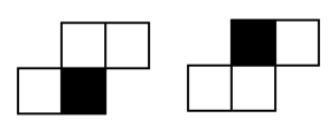
\includegraphics[scale=0.6]{imgs/2017-g1-2-p13-1.png}
\end{center}

\begin{center}
\begin{asy}
/* Math Kangaroo G1-2 2017 P13-1, revised by Teacher David */
size(4cm);
defaultpen(linewidth(0.7pt));

void plotbox(pair a, int flag) {
    pair b = a + (1,1);
    path x = box(a, b);
    
    if (flag == 0) {
        draw(x);
    } 
    else 
    {
        filldraw(x, heavygray);
    }
}

pair [] p = {(0,0), (1,1), (2,1), (4,0), (5,0), (6,1)};
for (int i=0; i<p.length; ++i) {
    plotbox(p[i], 0);
}

pair [] q = {(1,0), (5,1)};
for (int i=0; i<q.length; ++i) {
    plotbox(q[i], 1);
}

\end{asy}
\end{center}


The back is white. Which pattern can he make with those two tiles?
\begin{center}
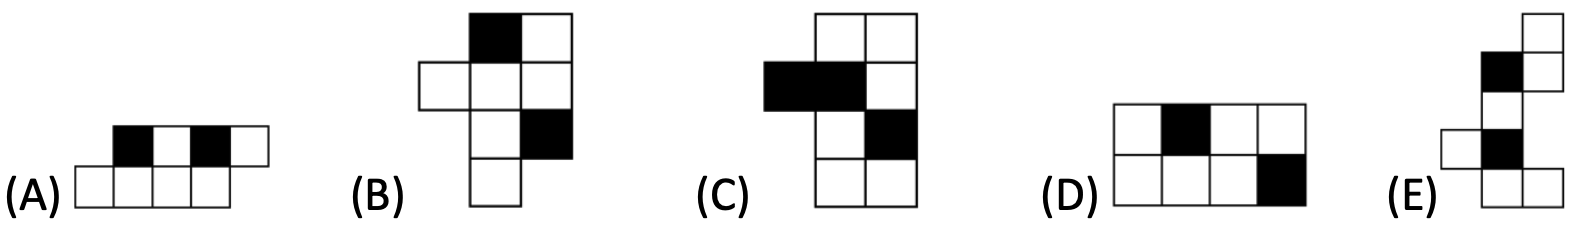
\includegraphics[scale=0.4]{imgs/2017-g1-2-p13-2.png}
\end{center}

\begin{center}
\begin{asy}
/* Math Kangaroo G1-2 2017 P13-2, revised by Teacher David */
size(14cm);
defaultpen(linewidth(0.7pt));

void plotbox(pair a, int flag) {
    pair b = a + (1,1);
    path x = box(a, b);
    
    if (flag == 0) {
        draw(x);
    } 
    else 
    {
        filldraw(x, heavygray);
    }
}

/* draw white boxes */
pair [] p = {(0,0), (1,0), (2,0), (3,0), (2,1), (4,1),
                  (8,2), (9,0), (9,1), (9,2), (10,2), (10,3),
                  (15,0),(15,1),(15,3), (16,0), (16,2), (16,3),
                  (20,0), (20,1), (21,0), (22,0), (22,1), (23,1),
                  (27,1), (28,0), (28,2), (29,0), (29,3), (29,4)};

for (int i=0; i<p.length; ++i) {
    plotbox(p[i], 0);
}

/* draw black boxes */
pair [] q = {(1,1), (3,1), (9,3), (10,1), (14,2), (15,2), (16,1), (21,1), (23,0), (28,1), (28,3)};
for (int i=0; i<q.length; ++i) {
    plotbox(q[i], 1);
}

/* add labels */
string [] s = {"(A)", "(B)", "(C)", "(D)", "(E)"};
pair [] a = {(2.5, -0.75), (9.5,-0.75), (15.5, -0.75), (22,-0.75), (28.5, -0.75)};
for (int i=0; i<s.length; ++i) {
    label(s[i], a[i]);
}
\end{asy}
\end{center}

$\text{(A) } \text{A} \qquad $$\text{(B) } \text{B} \qquad $$\text{(C) } \text{C}  \qquad $$\text{(D) } \text{D} \qquad $$\text{(E) } \text{E}$

\item (Math Kangaroo G3-4 2011, P21)  Andrea made the pattern in the picture out of several identical tiles. None of the tiles overlap each other. Which of the following tiles could she definitely not have used?

\begin{center}
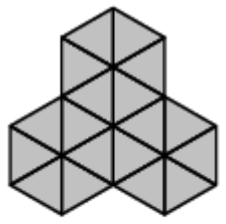
\includegraphics[scale=0.6]{imgs/2011-g3-4-p21-1.png}
\end{center}

\begin{center}
\begin{asy}
/* Math Kangaroo G3-4 2011 P21-1, revised by Teacher David */
size(4cm);
defaultpen(linewidth(1pt));

void plot(pair o) {
    path a = rotate(30)*polygon(6); /* hexagon at (0,0) */
    path b = shift(o)* a; /* shift hexagon to (o) */
    filldraw(b, gray); /* fill draw hexagon */

    for (int i=0; i<6; ++i) {
        pair x = o + dir(30+i*60);
        path p = o -- x;
        draw(p);
    }
}

pair a1 = (0,0);
plot(a1);

pair a2 = sqrt(3)*dir(-60);
plot(a2);

pair a3 = sqrt(3)*dir(-120);
plot(a3);
\end{asy}
\end{center}


\begin{center}
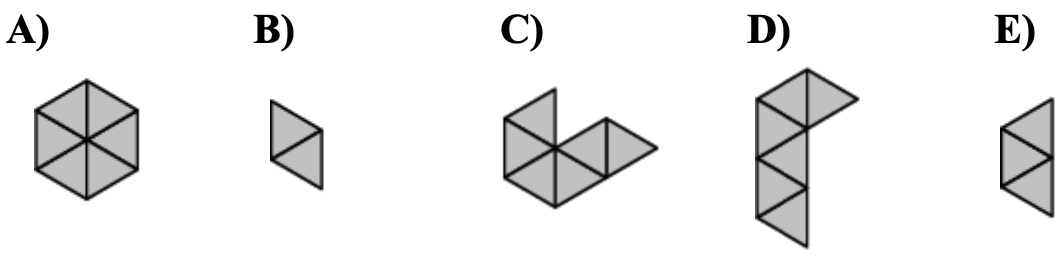
\includegraphics[scale=0.6]{imgs/2011-g3-4-p21-2.png}
\end{center}


\begin{center}
\begin{asy}
/* Math Kangaroo G3-4 2011 P21-1, revised by Teacher David */
size(12cm);
defaultpen(linewidth(1pt));

void plot(pair o, int start, int length) {
    for (int i=start; i<start+length; ++i) {
        int a1 = i*60 - 30;
        pair x = o+dir(a1);
        pair y = o+dir(a1+60);
        path p = o -- x -- y -- cycle;
        filldraw(p, gray);
    }
}
pair a1 = (0,0);
plot(a1, 0, 6);

pair a2 = (4,0);
plot(a2, 0, 2);

pair a3 = (8,0);
plot(a3, 2, 5);
pair a4 = (8+sqrt(3), 0);
plot(a4, 3, 1);

pair a5 = (12, 0);
plot(a5, 1, 4);
pair a6 = (12,-1);
plot(a6, 3, 2);

pair a7 = (16,0);
plot(a7, 2, 3);


/* add labels */
string [] s = {"(A)", "(B)", "(C)", "(D)", "(E)"};
pair [] a = {(0, 1.75), (4, 1.75), (8, 1.75), (12, 1.75), (16, 1.75)};
for (int i=0; i<s.length; ++i) {
    label(s[i], a[i]);
}

/* The original graph can also be plot in the following way:
pair a8 = (20,0);
plot(a8, 0, 6);
pair a9 = a8+sqrt(3)*dir(-60);
plot(a9, 0, 6);
pair a10 = a8+sqrt(3)*dir(-120);
plot(a10, 0, 6);
*/

\end{asy}
\end{center}


$\text{(A) } \text{A} \qquad $$\text{(B) } \text{B} \qquad $$\text{(C) } \text{C}  \qquad $$\text{(D) } \text{D} \qquad $$\text{(E) } \text{E}$


\end{enumerate}

\end{document}

